\expandafter\ifx\csname ifdraft\endcsname\relax
   \documentclass[a4j,12pt]{jsreport}
% 数式
\usepackage{amsmath,amsfonts}
\usepackage{bm}

% 画像
\usepackage[dvipdfmx]{graphicx}

% biblatex
\usepackage[style=numeric, sorting=none, maxbibnames=1000]{biblatex}
\addbibresource{graduation_thesis.bib}

%itembox
\usepackage{ascmac}
%breakitemboxのためのpackage
\usepackage{itembkbx}
% \usepackage{tcolorbox} 画像が見えなくなってしまう原因
% \usepackage{framed} 枠

%フォント
\usepackage[ipaex]{pxchfon}

\usepackage[top=35truemm,bottom=30truemm,left=30truemm,right=30truemm]{geometry}
\usepackage{float}
\usepackage{multicol}
\usepackage{multirow}
\usepackage{paralist}
\usepackage{caption}
%\captionsetup{format=plain, justification=centering} % キャプションを中央揃えにする
\usepackage{setspace}
\usepackage{algorithm}
\usepackage{algpseudocode}
\usepackage[dvipdfmx,hidelinks]{hyperref}
\usepackage{pxjahyper}
\usepackage{fancyhdr}
\usepackage{ltablex}
\usepackage{capt-of}
\usepackage{tabularx}
\usepackage{enumitem} % itemizeの行間 これは下になければならない
\usepackage{threeparttable} % 表の脚注


   \setlength{\headheight}{16.5pt}
   \captionsetup{format=hang}
   \begin{document}
   % 上部のヘッダー
\pagestyle{fancy}
\lhead{\rightmark}
\renewcommand{\chaptermark}[1]{\markboth{第\ \thechapter\ 章\ #1}{}}
\fi

\chapter{具体的活用とその考察}\label{chap:experiment}
本章でははじめに, 本システムをプロのストーリークリエーターに活用して頂いた具体的な活用事例について\ref{example}節で説明し, 取り組みを通じて得たアンケート結果とその考察, ログデータとその考察をそれぞれ\ref{quetionnaire_result}節, \ref{log}節で述べる. また, 筆者が行った提案に対する結果とその考察を\ref{self_result}節で述べる.
\section{具体的活用事例}\label{example}
\subsection{目的と概要}\label{outline}
本システムのストーリー創作支援における有用性を確かめる目的として, プロのストーリークリエーター数グループに, 本システムを利用してもらい, 商業誌, 週刊少年チャンピオン\footnotemark\footnotetext{\url{https://www.akitashoten.co.jp/w-champion} (cited 2024-01-27)} 2023年52号に掲載される『ブラック・ジャック』の新作エピソードのプロット制作に取り組んでもらった. 取り組みの中でアンケートの実施と操作ログの取得を行い, それらの分析を本取り組みの結果とした.

この取り組みを通じ, 本システムが提供する LLM の利用方法がプロの創作活動にどれだけの支援を与えるのか検証するとともに, LLM, ひいてはAIと人との共創のあり方とその可能性ついて探求した. なお, この取り組みは「TEZUKA2023プロジェクト」の一環として行われたものである.
\subsection{参加者}\label{purpose}
プロット制作に参加したグループとその構成を表\ref{group}に示す. 参加者はいずれもプロのクリエーターとして活動している.

\vspace*{-0.4cm}
\setlongtables
\begin{threeparttable}
   \begin{tabularx}{\textwidth}{ccccc}
      \caption[参加グループの構成]{参加グループの構成. \label{group}}
      \setlength{\belowcaptionskip}{-1pt}
      \vspace*{-0.2cm}
         \endfirsthead
   \hline
   グループ & 年齢 & 性別 & 創作活動歴\tnote{*} & ChatGPTの使用頻度\tnote{2}  \\ \hline
   A & 30代 & 女性 & 10年以上 & 月に数回使用する\\
   B & 60代 & 男性 & 30年以上 & 全く使用したことがない\\
   C & 40代 & 女性 & 20年以上 & ほとんど使用しない\\
   & 60代 & 男性 & - & ほとんど使用しない\\
   D & 60代 & 男性 & 40年以上 & 全く使用したことがない\\
   E & 60代 & 男性 & - & 全く使用したことがない \\
   & - & 女性 & - & \\
   \hline
   \end{tabularx}
   \vspace*{-0.5cm}
   \begin{tablenotes}\footnotesize
      \item[1] 創作活動歴については業界への参入年を参考にし不明なものは空欄とした. 
      \item[2] ChatGPTの使用頻度は5段階のリッカート尺度で取られたアンケート結果による.
   \end{tablenotes}
\end{threeparttable}
\vspace*{0.5cm}
%本研究では, 開発したアプリケーションの実践的な有用性を調査する目的として, プロのストーリークリエーターに, 出版誌に掲載する『ブラック・ジャック』の新作[TEZUKA 2023]のプロットを, 本アプリケーションを用いて制作してもらう実験を実施した.

\subsection{プロット制作期間とその流れ}\label{flow_of_plot}
プロット制作期間は「第1回プロット制作会議」が行われた2023年7月8日から「第2回プロット制作会議」が行われた2023年8月2日までのおよそ1ヶ月間であった. 正確に実施したアンケートは全部で3つ, 操作ログは本システムの利用における全編を通して取得した. 全体的な流れを表\ref{plot_flow}に示す.
\setlongtables
   \begin{tabularx}{\textwidth}{cc}
      \caption[具体的活用事例における全体の流れ]{具体的活用事例における全体の流れ \label{plot_flow}}
      \setlength{\belowcaptionskip}{-1pt}
      \vspace*{-0.2cm}
         \endfirsthead
   \hline
   \textbf{全体} & \textbf{実施項目} \\
   \hline
   第1回プロット制作会議 & 第1回アンケート実施 \\
   & $\downarrow$ \\
   & 主にプロット生成セクションの利用 \\
   & $\downarrow$ \\
   & 第2回アンケート実施 \\
   & $\downarrow$ \\
   各自プロット制作 & 主にプロット編集セクションの利用 \\
   & $\downarrow$ \\
   & プロットの完成 \\
   & $\downarrow$ \\
   第2回プロット制作会議 & プロット選定決議 \\
   & $\downarrow$ \\
   & 第3回アンケート実施 \\   
   \hline
   \end{tabularx}
\subsubsection{第1回プロット制作会議}
ここでは, 主に, プロット生成セクションの利用による各グループにとって初めてのプロット生成が行われ, そのことに関連した2つのアンケートを実施した. 以下ではその詳細について述べる.

第1回プロット制作会議は, 慶應義塾大学新川崎タウンキャンパス\footnotemark\footnotetext{\url{https://www.k2.keio.ac.jp/} (cited 2024-01-27)} にて全参加者が対面で集まり行われた. はじめに, 本取り組みの概要について参加者への説明を行い, アンケートを実施することと本システムの利用において操作ログを取得することについて全参加者から同意を得た. 次に, 参加者が本システムに触れる前に第1回目のアンケートを実施した. その内容を表\ref{quetionnaire_1}に示す. その後, 本システムの利用方法について大まかな説明を行い, 全参加者にとって初めての本システムの利用が行われた. 操作環境は, 1グループにつき1台のPCで, 当研究室の学生が各グループに一人アシスタントとしてついた.

利用されたのは主にプロット生成セクションであり, それぞれのグループにおいて, プロット生成セクションによる初めてのプロット生成が行われ, その後第2回目のアンケートを実施した. その内容を表\ref{quetionnaire_2}に示す.

その後, 各参加者が自身の好きな場所で本システムを用いたプロット制作が行えるよう, 本システムをそれぞれの参加者が持つPCへとセットアップし第1回プロット制作会議を終了した.

\subsubsection{第1回プロット制作会議終了から第2回プロット制作会議実施まで}
この期間各グループには自身の好きな場所で本システムを用いたプロット制作を行ってもらい, 第2回プロット制作会議に提出するためのプロットを完成させてもらった. このとき利用されたのは, プロット生成セクションに加え, 主にプロット編集セクションであった. なお, この期間本システムの利用において発生した不具合については, 本システムの開発者である当研究室の学生が対応した. 

\subsubsection{第2回プロット制作会議}
ここでは, 各グループが本システムを用い完成させたプロットの中から, 週刊少年チャンピオンに掲載する『ブラック・ジャック』の新作エピソードとして使われるプロットを1つ選定する決議が行われた. 決議には, プロット制作の参加者に加え, プロジェクトに参加している研究者, 出版社の担当者などが参加した. 決議において選定されたプロットを図\ref{plot_decided}に示す.

その後プロット制作を終えた各グループに対し第3回目のアンケートを実施した. その内容を表\ref{quetionnaire_3}に示す.

選定されたプロットは, 主に人の手による編集とシナリオ化が行われ, 最終的に週刊少年チャンピオン2023年52号に掲載される『ブラック・ジャック』の新作エピソードとして完成された. 選定されたプロットは次のとおり.

\begin{breakitembox}
   [l]{選定されたプロット}
   \noindent {シーン1: 依頼}\\
   1. 革新的なアンドロイド、“HeartBeat Mark II”が突如機能停止し、発明者である川村たかしがその解決の糸口を見つけられず困惑している。彼は自力では解決できず、ブラック・ジャックに助けを求める。(川村の視点)\\
   2. ブラック・ジャックはアンドロイドを人間のような存在として観察し、その心臓部分がただの機械部品で無く、生命体を理解する鍵であることを説明する。\\
   3. ブラック・ジャックは"HeartBeat Mark II"の心臓部分を調査し、心臓を制御する電子部品に異常があることを見つけ、それが機能停止の原因であることを明らかにする。そして、足元に広がりつつある全体のエネルギー供給の不安定さを川村に伝え、アンドロイドの生命の危険性を警告する。\\
   4. ブラック・ジャックの意見に対して、ドクター・キリコが口を開き、挑発する。彼の主張は"HeartBeat Mark II"が不安定になっているならば、何らかの危険を引き起こす可能性があるというものだった。この言葉が二人の間に対立の芽を生じさせる。\\
   5. 川村はドクター・キリコの主張に言葉を失い、混乱する。しかし"HeartBeat Mark II"の生命を守るために、ブラック・ジャックに全てを委ねる決断を下す。\\
   \\
   {シーン2: 危害}\\
   1. "HeartBeat Mark II"の生命を延長させたいブラック・ジャックは、ピノコがドクター・キリコに捕らえられたという警告の電話を受け、葛藤する。(ブラック・ジャックの視点)\\
   2. ブラック・ジャックはドクター・キリコの冷静さに怒り、アンドロイドの再起動に全力を尽くすことを誓う。\\
   3. しかし"HeartBeat Mark II"の心臓部分の異常を修正するには手術しかないとブラック・ジャックは結論付ける。\\
   4. 川村は、そのアンドロイドが人間の生命観に対する新たな視野を提供すること、そして科学と人間性の新たな境界を模索する中でその重要性を理解する。彼はブラック・ジャックが"HeartBeat Mark II"の生命を救うために手術することを支持し、その費用をすぐに提供する。\\
   5. しかし、その手術は革新的な機械科学の知識と技術を必要とし、特に心臓部分の修復は緻密で難解な作業だと分かる。不安に感じつつも、ブラック・ジャックはアンドロイドの問題を解決しようと意志を固める。\\
   6. その間も、ピノコは自らの命を救うために、ドクター・キリコによる拘束から逃れようと全力を尽くしている。\\
   \\
   {シーン3: 看病・治療}\\
   1. ブラック・ジャックは川村の信頼と"HeartBeat Mark II"の心臓部分の”生命”を信じて、冷静に複雑な手術に挑む。(ブラック・ジャックの視点)\\
   2. 手術は難関だった。微細な機械構造と専門的な技術が求められる"HeartBeat Mark II"の心臓部分の手術を進めるブラック・ジャック。彼の専門知識の欠如が手術の難易度をさらに上昇させる。\\
   3. しかし、ブラック・ジャックの不屈の努力はやがて結果を伴い、心臓部分の異常は修正され、手術は成功する。\\
   4. ピノコが自力で逃げようとする。その時、ドクター・キリコの部屋からうめき声が聞こえる。\\
   5. 脱出したピノコがドクター・キリコの部屋に来る。ドクター・キリコが胸を押さえて苦しそうにもがいている。そして、気を失う。それを見たピノコがドクター・キリコの異変に驚き、ブラック・ジャックに電話する。\\
   \\
   {シーン4: 変革}\\
   1. ブラック・ジャックがドクター・キリコを診察している。ブラック・ジャック「心臓だ！緊急オペを行う。」ピノコが手伝う。\\
   2. 診察台に眠っているドクター・キリコ。ブラック・ジャックはその胸を切開する。その心臓を見て、ブラック・ジャックは驚く。\\
   3. なんと！ドクター・キリコの心臓は、アンドロイドの心臓だった。ブラック・ジャックはそれを手術する。\\
   4. 数日後、ドクター・キリコが目を覚ます。ブラック・ジャックを見て、「何でお前がここに？」ブラック・ジャック「お前に緊急のオペが必要だったんでね。」ドクター・キリコ「何故死なせてくれなかった？」ブラック・ジャック「命を救うのが医者だからな。」ドクター・キリコ「俺はそうは思わない。」ブラック・ジャック「絶対安静だ。しばらく静かにしていろ。安心しろ、オペは確かだから。」と言って去る。ドクター・キリコ「アンドロイドプロジェクトなんて、俺が必ず壊してやる！」と叫ぶ。\\
   \\
   {シーン5: エピローグ}\\
   1. 去っていくブラック・ジャックとピノコ。ピノコ「せんせい、本当のことを言わなくていいの？」それに応えず、歩き続けるブラック・ジャック。それについていくピノコ。（終わり）\\
   
\end{breakitembox}
\vspace*{-7pt}
\begingroup
\captionof{figure}{選定されたプロット}
\label{plot_decided}
\endgroup

その他の提出されたプロットに関しては付録\ref{app:plot}に示す.

\subsection{アンケートの内容}\label{quetionnaires}
正確に実施されたアンケートは全部で3つあり, それらを以下の表\ref{quetionnaire_1}、\ref{quetionnaire_2}、\ref{quetionnaire_3}に示す. なおアンケートはいずれもGoogleフォーム\footnotemark\footnotetext{\url{https://www.google.com/intl/ja_jp/forms/about/} (cited 2024-01-27)} を用いて実施した.

アンケートの内容については, 筆者と他1名の学生が担当し, Measuring Narrative Engagement\cite{busselle09}などを参考に作成した.

本システムの利用を前に実施した第1回目のアンケートでは, 主にAIへの馴染み深さと期待度について尋ね, プロット生成セクションの利用を終えたのちに実施した第2回目のアンケートでは、主に生成されたプロットに対する満足度と『ブラック・ジャック』らしさ, プロットの制御性について尋ね, プロット編集セクションの利用も終え, プロットを完成させたのちに実施した第3回目のアンケートでは, 主に完成したプロットに対する満足度と『ブラック・ジャック』らしさ, プロットの制御性, 編集セクションの効果および創作活動における利便性について尋ねた.

\newcolumntype{Y}{>{\centering\arraybackslash}X} % 中央揃えのX列タイプを定義

\setlongtables
\begin{tabularx}{0.8\textwidth}{Yc}
   \caption[第1回目のアンケート内容]{第1回目のアンケート内容. \label{quetionnaire_1}}
   \setlength{\belowcaptionskip}{-1pt}
   \vspace*{-0.2cm}
   \endfirsthead
   \hline
   \textbf{質問内容} & \textbf{回答形式} \\
   \hline
   ChatGPTの使用頻度 & 5段階のリッカート尺度 \\
   ChatGPTの使用用途 & 自由記述 \\
   創造的作業におけるAIへの期待値 & 5段階のリッカート尺度 \\
   AIに期待していること & 自由記述 \\
   「ブラック・ジャック」新作について、\newline 現時点において持つアイデア & \multirow{2}{*}{自由記述} \\
   \hline
\end{tabularx}

\setlongtables
\begin{tabularx}{\textwidth}{Ycc}
   \caption[第2回目のアンケート内容]{第2回目のアンケート内容. \label{quetionnaire_2}}
   \setlength{\belowcaptionskip}{-1pt}
   \vspace*{-0.2cm}
   \endfirsthead
   \hline
   \textbf{質問内容} & \textbf{項目} & \textbf{回答形式} \\
   \hline
   『ブラック・ジャック』らしさ & 物語の展開 & 5段階のリッカート尺度 \\
   & 既存キャラ & 5段階のリッカート尺度 \\
   & 新規キャラ & 5段階のリッカート尺度 \\
    『ブラック・ジャック』らしい要素 & \multirow{2}{*}{-} & \multirow{2}{*}{自由記述} \\
    『ブラック・ジャック』らしくない要素 & \multirow{2}{*}{-} & \multirow{2}{*}{自由記述} \\
    既存エピソードとの類似性 & - & 3段階のリッカート尺度 \\
    上記で過度に類似していた部分 & - & 自由記述 \\
    物語のクオリティ & 一貫性 & 5段階のリッカート尺度 \\
    & 新規性 & 5段階のリッカート尺度 \\
    & 展開の起伏 & 5段階のリッカート尺度 \\
    & 思いつかない展開か & 5段階のリッカート尺度 \\
    & 内容の幅広さ & 5段階のリッカート尺度 \\
    & 総合的な面白さ & 5段階のリッカート尺度 \\
    クオリティについて感じたこと & - & 自由記述 \\
    入力内容の反映 & ジャンル & 5段階のリッカート尺度 \\
    & テーマ & 5段階のリッカート尺度 \\
    & アイデア & 5段階のリッカート尺度 \\
    & 物語構造 & 5段階のリッカート尺度 \\
    & 登場人物の属性 & 5段階のリッカート尺度 \\
    & 登場人物の性格 & 5段階のリッカート尺度 \\
    & 世界観(時代・場所) & 5段階のリッカート尺度 \\
    各シーンの物語構造との合致 & 各シーン & 5段階のリッカート尺度 \\
    上記が合致していない場合 \newline 相応しい名称 & \multirow{2}{*}{-} & \multirow{2}{*}{自由記述} \\
   \hline
\end{tabularx}

\setlongtables
\begin{tabularx}{\textwidth}{Ycc}
   \caption[第3回目のアンケート内容]{第3回目のアンケート内容. \label{quetionnaire_3}}
   \setlength{\belowcaptionskip}{-1pt}
   \vspace*{-0.2cm}
   \endfirsthead
   \hline
   \textbf{質問内容} & \textbf{項目} & \textbf{回答形式} \\
   \hline
   『ブラック・ジャック』らしさ & 物語の展開 & 5段階のリッカート尺度 \\
   & 既存キャラ & 5段階のリッカート尺度 \\
   & 新規キャラ & 5段階のリッカート尺度 \\
    『ブラック・ジャック』らしい要素 & \multirow{2}{*}{-} & \multirow{2}{*}{自由記述} \\
    『ブラック・ジャック』らしくない要素 & \multirow{2}{*}{-} & \multirow{2}{*}{自由記述} \\
    既存エピソードとの類似性 & - & 3段階のリッカート尺度 \\
    上記で過度に類似していた部分 & - & 自由記述 \\
    物語のクオリティ & 一貫性 & 5段階のリッカート尺度 \\
    & 新規性 & 5段階のリッカート尺度 \\
    & 展開の起伏 & 5段階のリッカート尺度 \\
    & 思いつかない展開か & 5段階のリッカート尺度 \\
    & 内容の幅広さ & 5段階のリッカート尺度 \\
    & 総合的な面白さ & 5段階のリッカート尺度 \\
    クオリティについて感じたこと & - & 自由記述 \\
    入力内容の反映 & ジャンル & 5段階のリッカート尺度 \\
    & テーマ & 5段階のリッカート尺度 \\
    & アイデア & 5段階のリッカート尺度 \\
    & 物語構造 & 5段階のリッカート尺度 \\
    & 登場人物の属性 & 5段階のリッカート尺度 \\
    & 登場人物の性格 & 5段階のリッカート尺度 \\
    & 世界観(時代・場所) & 5段階のリッカート尺度 \\
    各シーンの物語構造との合致 & 各シーン & 5段階のリッカート尺度 \\
    上記が合致していない場合 \newline 相応しい名称 & \multirow{2}{*}{-} & \multirow{2}{*}{自由記述} \\
    追加指示の反映 & - & 5段階のリッカート尺度 \\
    作業時間の短さ & - & 5段階のリッカート尺度 \\
    使いやすさ & - & 5段階のリッカート尺度 \\
    編集指示が反映された部分 \newline 反映されなかった部分 & \multirow{2}{*}{-} & \multirow{2}{*}{自由記述} \\
    使いやすかった機能 & - & 自由記述 \\
    使いにくかった機能および \newline ほしい機能 & \multirow{2}{*}{-} & \multirow{2}{*}{自由記述} \\
    編集作業後面白くなったか & - & 5段階のリッカート尺度 \\
    本システムの総合的な満足度 & - & 5段階のリッカート尺度 \\
    創造性を刺激されたか & - & 5段階のリッカート尺度 \\
    その他の意見 & - & 自由記述 \\
    創作活動における \newline AIとの理想な付き合い方 &\multirow{2}{*}{-} & \multirow{2}{*}{自由記述} \\
   \hline
\end{tabularx}

\subsection{操作ログの取得内容}
操作ログは, 参加者が本システムのなかでページにアクセスしたとき(GET)とデータを送信したとき(POST)に都度記録される仕組みである. 操作ログの項目は以下の表\ref{tab:log}に示すとおり.

\setlongtables
\begin{tabularx}{\textwidth}{cc}
   \caption{操作ログの項目 \label{tab:log}}
   \setlength{\belowcaptionskip}{-1pt}
   \vspace*{-0.2cm}
   \endfirsthead
   \hline
   \textbf{項目名} & \textbf{内容} \\
   \hline
   id & id番号\\
   timestamp & 記録された時刻(秒単位)\\
   request & GET or POST\\
   url & アクセスされたページのURL\\
   input & ユーザーの入力内容およびボタン名\\
   output & GPT-4からの出力内容\\
   settings & 設定ファイル\\
   latest\_plot & 最新のプロット\\
   latest\_scenario & 最新のシナリオ\\
   \hline
\end{tabularx}

\section{アンケートの分析結果および考察}\label{quetionnaire_result}
ここでは, 各項, 取り組みのなかで実施した3つのアンケートそれぞれについて分析結果を示しその考察を述べる.

なお, アンケートの分析においては, 筆者と他1名の学生で取り組んだ.

\subsection{第1回目のアンケート}\label{before}
第1回目のアンケートは, 本システムを利用してもらう前に実施したアンケートである. このアンケートでは, 主にAIへの馴染み深さと期待度について尋ねた. 以下ではその分析結果を示し考察を述べる.

\subsubsection{AIへの期待度および使用頻度}
創作活動におけるAIへの期待度に関する分析結果を図\ref{expectation}に示す. 図\ref{expectation}より, この時点において半数以上のグループがAIに対し高い期待を持っていたことが分かる.

これは昨今のAIの急速な発展における認知度の拡大と注目度の高さを反映した結果であると考えられる.
\begin{figure}[hbtp]
   \begin{center}
   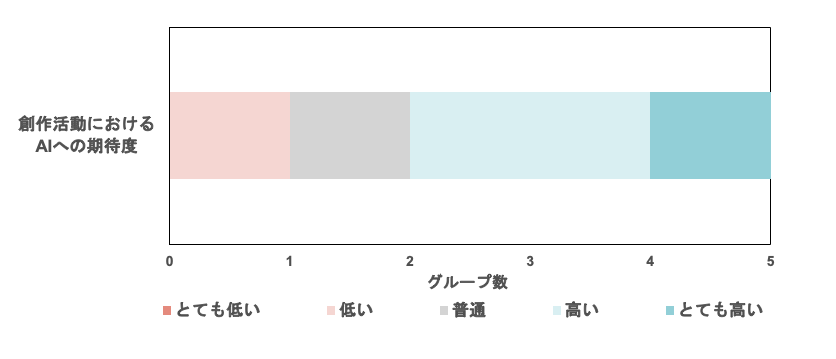
\includegraphics[width=12cm]{pict/05/expectation.png}
   \caption[AIへの期待度]{AIへの期待度.\footnotesize 第1回目のアンケートにおける「創造的作業におけるAIへの期待値はどれほどでしょうか？」という質問に対する回答結果}
   \label{expectation}
   \end{center}
\end{figure}
\vspace*{-0.3cm}

次に, ChatGPTの使用頻度に関する分析結果を図\ref{ChatGPT_Frequency}に示す. 図\ref{ChatGPT_Frequency}より, プロジェクトに参加したプロのストーリークリエーターの多くがこの時点において ChatGPT をほとんど使用していなかったことが分かる. 

これは, 図\ref{expectation}の結果とは対照的な結果であり, このことから, 参加したクリエーターは, AIに期待を持ちながらもその使用には消極的な姿勢を持っていたと解釈される. 図\ref{expectation}に示した結果も踏まえ, この結果は, ChatGPT含め, AIの発展等については報道などで触れる機会はありつつも, 実際自分自身の手で触れることにはまだまだ参入障壁となるハードルが存在していることを示唆する結果であるといえる.


\begin{figure}[hbtp]
   \begin{center}
   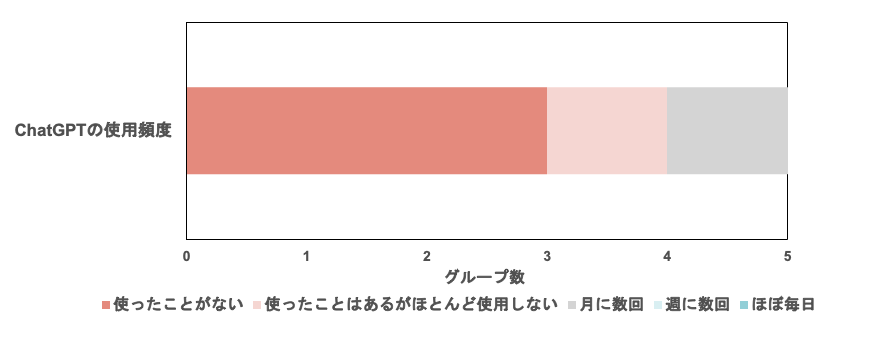
\includegraphics[width=12cm]{pict/05/ChatGPT_Frequency.png}
   \caption[ChatGPTの使用頻度.]{ChatGPTの使用頻度. \footnotesize 第1回目のアンケートにおける「あなたのChatGPTの使用頻度を教えてください。」という質問に対する回答結果}
   \label{ChatGPT_Frequency}
   \end{center}
\end{figure}

次に, ChatGPTの使用頻度とAIへの期待度の関係を示した散布図を図\ref{frequency-expectation}に示す. 図\ref{frequency-expectation}より, ChatGPTの使用頻度が低い, 利用経験がほとんどないグループほどAIへの期待度が高く, ChatGPTの使用頻度がそれなりにあるグループでは, AIへの期待度が低いことが分かる. このことから, ChatGPTを使用しないグループはその背景に, 性能に対する疑念とそれによる期待の欠如ではなく, その他の参入障壁を抱えていることなどが推察される. たとえば, 彼らにとって使い方が不明確, 不明瞭であるという点などが挙げられる. 一方で、ChatGPTをそれなりに使用した経験を持つと回答したグループにおいてAIへの期待度が比較的低いその理由としては, これまでクリエーター自身の一般的な使い方では十分に満足のいく結果を得られていない経験をもつことなどが背景にあると推察される.

本システムは, このようなAIに対する参入障壁を取り除くとともに, 有益な利用方法を提供することで創作活動におけるAIの活用を促進することを目的としている.


\begin{figure}[hbtp]
   \begin{center}
   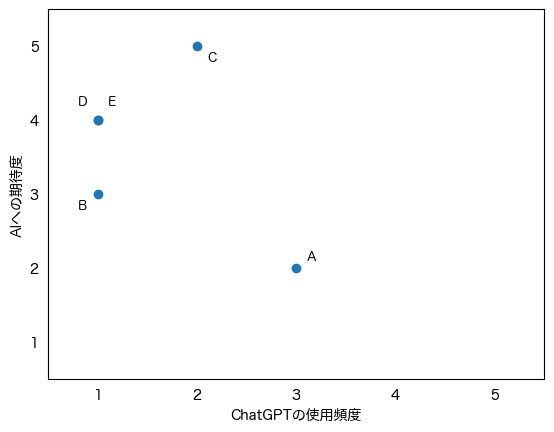
\includegraphics[width=10cm]{pict/05/frequency-expectation.png}
   \caption{ChatCPTの使用頻度とAIへの期待度の関係}
   \label{frequency-expectation}
   \end{center}
\end{figure}

\subsubsection{制作を前に思いつくアイデア}
表\ref{tab:expectation}に, 制作を前に思いつく限り記述してもらった『ブラック・ジャック』のアイデアをグループごとに全て示す.  表\ref{tab:expectation}より, 『ブラック・ジャック』の新作エピソードに用いるアイデアとして, 過去の作品である『ブラック・ジャック』に現代性を取り入れようとするアイデアが半数以上のグループで挙げられていたことが分かる. 

これは, 新作エピソードとして, 『ブラック・ジャック』の世界観の継承を, 『ブラック・ジャック』の物語構造分析に基づく本システムの利用をもって担保し, その上で現代の社会情勢を反映させることで, 『ブラック・ジャック』の新たな魅力を引き出すことができるのではないかという期待の表れであると考えられる. 

実際週刊少年チャンピオンに掲載された『ブラック・ジャック』の新作エピソードは, 『ブラック・ジャック』の世界観の継承と現代の社会情勢の反映を両立させたものであるとして評価を受けた. AI との創作活動において, 時代を越えた作品作りの実現に期待が寄せられていると考えられる.

% 次に, 本システムを用いた『ブラック・ジャック』の新作エピソードの制作を前に, 考えられるアイデアを思いつく限り記述してもらったアンケート結果を表\ref{tab:expectation}に示す. 表\ref{tab:expectation}より, 『ブラック・ジャック』の新作エピソードに用いるアイデアとして, 過去の作品である『ブラック・ジャック』に現代性を取り入れようとするアイデアが半数以上のグループで挙げられていたことが分かる. 
% \vspace*{0.2cm}

\vspace{5cm}

\begin{tabularx}{12cm}{X}
   \caption[制作を前に記述されたアイデア.]{制作を前に記述されたアイデア. \footnotesize 第1回目のアンケートにおける「『ブラック・ジャック』の新作について、現時点で思いつくアイデアを箇条書きでできるだけ列挙してください。展開や単語など内容はなんでも構いません。」という質問に対する回答結果 \label{tab:expectation}}
   \vspace{-5pt}
   \endfirsthead
   \hline
   \vspace{0.2cm}
   \begin{minipage}{\linewidth}
      \vspace{0.1cm}
         \begin{itemize}[itemsep=0pt, parsep=2pt]
            \item グループA:
               \begin{itemize}[itemsep=0pt, parsep=5pt]
                  \item 血縁的な家族ではなくても家族である、的な現代らしい人間関係のとらえなおしを扱う。
                  \item 原発など、手塚先生ご存命の時とは世の中のとらえ方が変わったものを扱う。
                  \item ジェンダーや世代を超えたキャラクター作りがどこまでいけるのか。
                  \item 価値観を揺さぶるもの。
            \end{itemize}
         \end{itemize}
   \end{minipage} \\
   \begin{minipage}{\linewidth}
      \vspace{0.2cm}
         \begin{itemize}[itemsep=0pt, parsep=2pt]
            \item グループB:
               \begin{itemize}[itemsep=0pt, parsep=5pt]
                  \item 体のほとんどの骨が手術により、チタンになった男の話
               \end{itemize}
         \end{itemize}
   \end{minipage} \\
   \begin{minipage}{\linewidth}
      \vspace{0.5cm}
         \begin{itemize}[itemsep=0pt, parsep=2pt]
            \item グループC:
               \begin{itemize}[itemsep=0pt, parsep=5pt]
                  \item 社会テーマ
                  \item パニックサスペンス
                  \item ヒューマンドラマ
               \end{itemize}
         \end{itemize}
   \end{minipage} \\
   \begin{minipage}{\linewidth}
      \vspace{0.5cm}
         \begin{itemize}[itemsep=0pt, parsep=2pt]
            \item グループD:
               \begin{itemize}[itemsep=0pt, parsep=5pt]
                  \item もしブラックジャックが現代にいたら何をするか。
               \end{itemize}
         \end{itemize}
   \end{minipage} \\
   \begin{minipage}{\linewidth}
      \vspace{0.5cm}
         \begin{itemize}[itemsep=0pt, parsep=2pt]
            \item グループE:
               \begin{itemize}[itemsep=0pt, parsep=5pt]
                  \item 人情話
                  \item 現代の医療器具の使用
               \end{itemize}
         \end{itemize}
         \vspace{0.5cm}
   \end{minipage} \\
   \hline
\end{tabularx}

\subsection{第2回目のアンケート}\label{after}
第2回目のアンケートは, 本システムのプロット生成セクションの利用を終えたのちに実施したアンケートである. このアンケートでは, 主に生成されたプロットに対する満足度と『ブラック・ジャック』らしさ, システムの操作性について尋ねた. 以下ではそれらの分析結果を示しその考察を述べる.

\subsubsection{初回プロットにおける『ブラック・ジャック』らしさ}
初回に生成されたプロットにおいて, 『ブラック・ジャック』らしさがどれだけ表れていたか尋ねたアンケート結果を図\ref{similarity}に示す. 図\ref{similarity}より, 本システムのプロット生成セクションの利用により, いずれの項目においてもプロのストーリークリエーターの視点から『ブラック・ジャック』らしいと感じられるプロットの生成が, 概ね行われていたことが分かる. これは, 本システムにおける『ブラック・ジャック』の物語構造分析の活用が, 『ブラック・ジャック』の世界観の継承の確保に寄与することを示唆する結果であるといえる. また, 各参加者にとって, 本システムの利用の初回にも関わらず『ブラック・ジャック』らしさを持つプロットが生成できたと, 多くのグループに思われたことは, 本システムのプロット生成セクションの利用における操作性の高さ, 物語構造分析を活用したことによる優位性の高さを示唆する結果であると考えられる.
%本システムのプロット生成セクションの利用により, いずれの項目においてもプロのストーリークリエーターの視点から『ブラック・ジャック』らしいと感じられるプロットの生成が行われたということがわかる.
%本システムのプロット生成セクションは, いずれの項目においても, プロのストーリークリエーターに『ブラック・ジャック』らしいと感じられるプロットを生成していたことが分かる.
%いずれの項目においても多くのプロのストーリークリエーターに, 生成されたプロットの中で『ブラック・ジャック』らしさが感じられたと評価されていることが分かる.

\begin{figure}[H]
   \begin{center}
   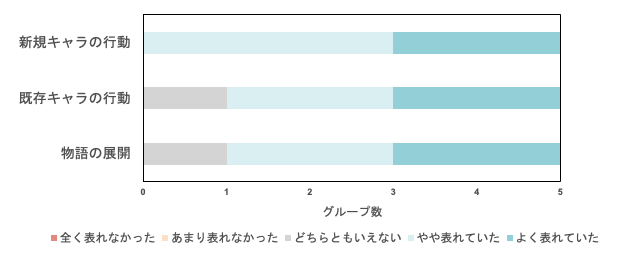
\includegraphics[width=12cm]{pict/05/similarity.png}
   \caption[初回プロットにおける『ブラック・ジャック』らしさ]{ 初回プロットにおける『ブラック・ジャック』らしさ \footnotesize 第2回目のアンケートにおける「『ブラック・ジャック』らしさをどの程度感じたか教えてください。」という質問に対する回答結果\label{similarity}}
   
   \end{center}
\end{figure}
\vspace{-0.5cm}

次に, 初回に生成されたプロットで『ブラック・ジャック』らしさが感じられた要素を自由に記述してもらったアンケート結果を表\ref{tab:similarity}に示す. 表\ref{tab:similarity}より, 『ブラック・ジャック』らしさが感じられた要素としてキャラクターに関する要素と物語展開に関する要素どちらについても言及されていることが分かる. これは, 本システムのプロット生成セクションにおける物語構造分析の活用として, 物語展開の分析とキャラクター分析の活用そのいずれもが, LLM の制御として効果的に働くことを示唆する結果であるとえる.

%『ブラック・ジャック』らしさが感じられた要素としてキャラクターに関する要素と物語展開に関する要素, どちらについても言及されていることが分かる. これは, 
% ここでの記述はキャラクターに関する要素と物語展開に関する要素に分類され, 本システムのプロット生成セクションの利用が, どちらの要素についても『ブラック・ジャック』らしい要素として表すプロットの生成を可能にしたことが分かる. このことは, 本システムのプロット生成セクションにおける物語構造分析の活用として, 物語展開の分析とキャラクター分析の活用そのいずれもが, LLM の制御として効果的に働くことを示唆する結果であるとえる.

\vspace*{0.5cm}

\begin{tabularx}{12cm}{X}
   \caption[初回たプロットにおいて『ブラック・ジャック』らしさが感じられた要素.]{初回プロットにおいて『ブラック・ジャック』らしさが感じられた要素. \footnotesize 第2回目のアンケートにおける「『ブラック・ジャック』らしさがよく表れていた要素（物語展開やキャラの行動）があれば教えてください。」という質問に対する回答結果 \label{tab:similarity}}
   \vspace{-5pt}
   \endfirsthead
   \hline
   \vspace{0.2cm}
   \begin{minipage}{\linewidth}
      \vspace{0.1cm}
         \begin{itemize}[itemsep=0pt, parsep=2pt]
         \item グループA:
            \begin{itemize}[itemsep=0pt, parsep=2pt]
               \item 現実離れした、でも「この世のどこかには必ずありそう」な場所設定とキャラの展開。
            \end{itemize}
         \end{itemize}
   \end{minipage} \\
   \begin{minipage}{\linewidth}
      \vspace{0.2cm}
         \begin{itemize}[itemsep=0pt, parsep=2pt]
         \item グループB:
            \begin{itemize}[itemsep=0pt, parsep=2pt]
               \item 機械の心臓を手術する
            \end{itemize}
         \end{itemize}
   \end{minipage} \\
   \begin{minipage}{\linewidth}
      \vspace{0.5cm}
         \begin{itemize}[itemsep=0pt, parsep=2pt]
         \item グループC:
            \begin{itemize}[itemsep=0pt, parsep=2pt]
               \item 既存キャラクターの役回り
            \end{itemize}
         \end{itemize}
   \end{minipage} \\
   \begin{minipage}{\linewidth}
      \vspace{0.5cm}
         \begin{itemize}[itemsep=0pt, parsep=2pt]
         \item グループD:
            \begin{itemize}[itemsep=0pt, parsep=2pt]
               \item 裏切りが効果的に使われていた。
            \end{itemize}
         \end{itemize}
   \end{minipage} \\
   \begin{minipage}{\linewidth}
      \vspace{0.5cm}
         \begin{itemize}[itemsep=0pt, parsep=2pt]
         \item グループE:
            \begin{itemize}[itemsep=0pt, parsep=2pt]
               \item 岡崎にたいする態度
            \end{itemize}
         \end{itemize}
         \vspace{0.2cm}
   \end{minipage} \\
   \hline
\end{tabularx}

\subsubsection{初回プロットの満足度}

初回に生成されたプロットに対する各項目のクオリティについて尋ねたアンケート結果を図\ref{quality}に示す. 図\ref{quality}より, 本システムのプロット生成セクションの利用は, 生成されるプロットに一貫性を作り出すという観点においてはまずまずの回答を得た一方, 一貫性を除くその他多くの項目では, 良いという意見と悪いという意見が拮抗し, 十分に良さを与えるものとしてはみなされなかったことが分かる. このことは, 本システムにおける物語構造分析の活用においてその活用は, 一貫性, つまり矛盾なく物語が展開されることにそれなりの寄与を与えるものの, 既存の物語に対する分析を活用していることにより, 幅広さや新規性などといった面で生成物に十分なクオリティをもたらすことは難しいということを示唆する結果であるといえる. また, 新規性や思いつかない展開を含むプロットを生成できていないと思われた点については, 出力が学習データに左右される LLM を物語の創作に活用する上で重要な課題の一つであるということができる.

%本システムのプロット生成セクションの利用により, 一貫性においてはまずまずのプロットが生成された一方, 一貫性を除くその他多くの項目で, 良い評価と悪い評価が拮抗するようなプロットが生成されてしまったことが分かる.

%図\ref{quality}より, 生成されたプロットのクオリティについて, 一貫性を除いた多くの項目で良くないという評価と良いという評価が拮抗していることが分かる.

\begin{figure}[H]
   \begin{center}
   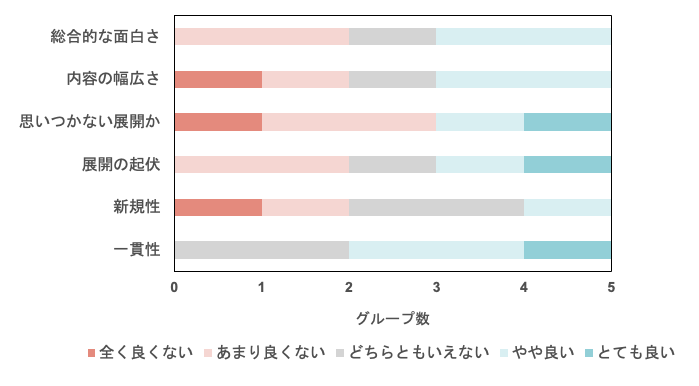
\includegraphics[width=12cm]{pict/05/quality.png}
   \caption[初回プロットに対するクオリティについての回答]{初回プロットに対するクオリティについての回答 \footnotesize 第2回目のアンケートにおける「物語としてのクオリティについて評価してください。」という質問に対する回答結果 \label{quality}}
   \end{center}
\end{figure}

次に, 図\ref{quality}において示した回答をグループごとにまとめ, 図\ref{quality_g}に示す. ここでは, 1 から 5 の数字 が「全く良くない」から「とても良い」を順に表す. 図\ref{quality_g}より, どのグループにおける回答についても項目間にそれほど大きなばらつきが見られないことが分かる. つまり, ある項目で低い評価をつけるグループは他の項目についても低い評価を, ある項目で高い評価をつけるグループは他の項目でも高い評価をつけていたことが分かる. このことから, 生成されるプロットにおいてこれらの項目は互いに相関を持っている可能性があること, 評価はグループごとの判断基準の違いに大きく依存すること, 生成されるプロットはグループごと, つまり設定ごと, 出力ごとに質の差が生まれてしまうことなどが考えられる.

\begin{figure}[H]
   \begin{center}
   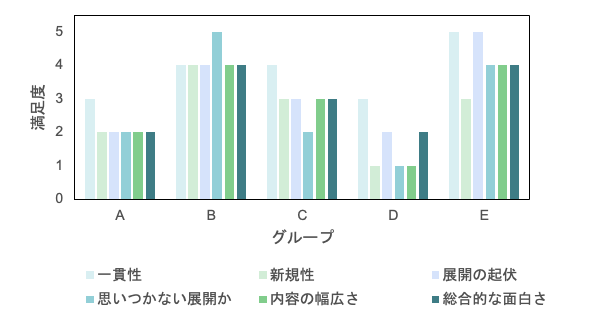
\includegraphics[width=12cm]{pict/05/quality_g.png}
   \caption[プロットのクオリティに対するグループごとの回答]{プロットのクオリティに対するグループごとの回答. \footnotesize 1 から 5 の数字は「全く良くない」から「とても良い」を順に表す.}
   \label{quality_g}
   \end{center}
\end{figure}

\subsubsection{初回プロットに対する制御性}

プロット生成セクションにおいて設定した内容が, 生成されたプロットにどれだけ反映されたかその反映具合について尋ねたアンケート結果を図\ref{control}に示す. 図\ref{control}より, 本システムのプロット生成セクションの利用は, 物語構造, 登場人物の性格, 属性においてはその設定をよくプロットに反映させることができていたと分かる. これは, 物語構造分析における物語展開の分析の活用とキャラクター分析の活用が, 本システムのプロット生成セクションにおいて有効に働いたことに起因する結果であると考えられる. 一方で, テーマにおいてはその設定を十分にプロットの中に反映させることができていないとみなされた. これは, 先ほどの図\ref{quality}において示したプロットのクオリティにおいて高い評価を得られなかった原因の一つとして考えることができる. つまり本システムのプロット生成セクションにおいては, 物語構造分析におけるキャラクター分析を活用した登場人物の設定や物語展開の活用が物語の一貫性や『ブラック・ジャック』らしさを担保する上で有効であるものの, 現代性など, 作品ごとに与える新たなテーマを反映させることには不十分であり, 新規性や幅広さといった面で満足を与えるクオリティを持つプロットを生成することが難しくなっているといったことが推察される.

%本システムのプロット生成セクションの利用は, 生成されるプロットの中に, 物語構造, 登場人物の性格, 属性の設定をよく反映させていたことが分かる

\begin{figure}[H]
   \begin{center}
   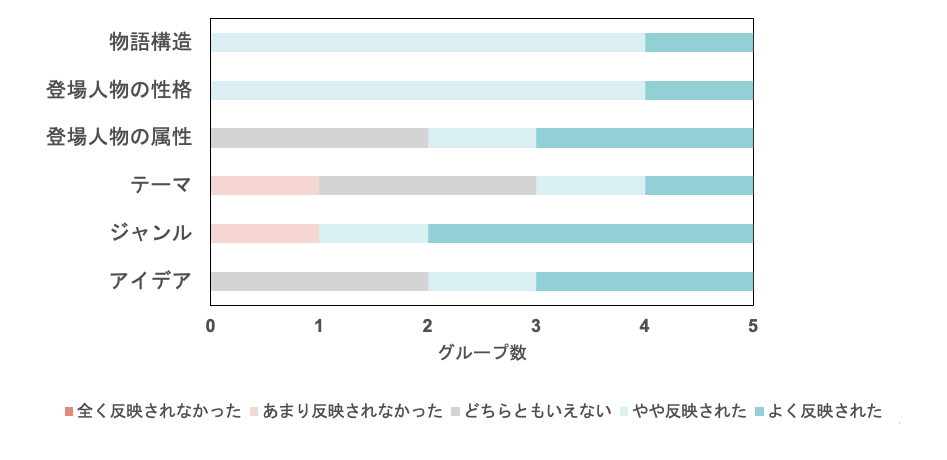
\includegraphics[width=12cm]{pict/05/control.png}
   \caption[初回プロットの制御性に関するアンケート結果]{初回プロットの制御性に関するアンケート結果 \footnotesize 第2回目のアンケートにおける「入力内容が出力プロットにどれほど反映されたと感じますか？」という質問に対する回答結果 \label{control}}
   \end{center}
\end{figure}

\subsection{第3回目のアンケート}
第3回目のアンケートは, 第2回プロット制作会議におけるプロット選定決議を終えた後, つまり, 各グループがプロット編集セクションの利用も含めてプロットの制作を終えたのちに実施したアンケートである. このアンケートでは, 主に制作されたプロットに対する満足度と『ブラック・ジャック』らしさ, プロットの制御性, 編集セクションの効果および創作活動における利便性について尋ねた. 以下ではそれらの分析結果を示しその考察を述べる.
% ここでは, 第2回プロット制作会議におけるプロット選定決議を終えた後, つまり, 各グループがプロット編集セクションの利用も含め, 本システムを活用し, 会議に提出するためのプロットの制作を完了させた後に実施したアンケート結果を示し, その考察を行う.

\subsubsection{制作されたプロットの『ブラック・ジャック』らしさ}
制作されたプロットにおいて, 『ブラック・ジャック』らしさについて尋ねたアンケート結果を図\ref{similarity2}に示す. 図\ref{similarity2}より, 本システムの活用により制作されたプロットは, プロのストーリークリエーターから見て概ねどの項目についても『ブラック・ジャック』らしさをもつとみなされていることが分かる. 図\ref{similarity}においてもよく『ブラック・ジャック』らしさが感じられていたことを踏まえると, プロット編集セクションの利用は, プロット生成セクションにおいて生み出された『ブラック・ジャック』らしさを損なうことにはならないことを示唆する結果であると考えられる. これらの結果は, 本システムの活用がプロのストーリークリエーターを基準に『ブラック・ジャック』らしさを持つと判断されるプロット制作に効果的であることを示唆する結果であるといえる.

%図\ref{similarity2}より, 図\ref{similarity}に示した, 第一回目に生成されたプロットにおける『ブラック・ジャック』らしさの評価同様, どの項目についても, 編集セクション含め本システムを利用し完成されたプロットの中に『ブラック・ジャック』らしさが表れていたとプロのストーリークリエーターから概ね高い評価を得ることができた.

\begin{figure}[H]
   \begin{center}
   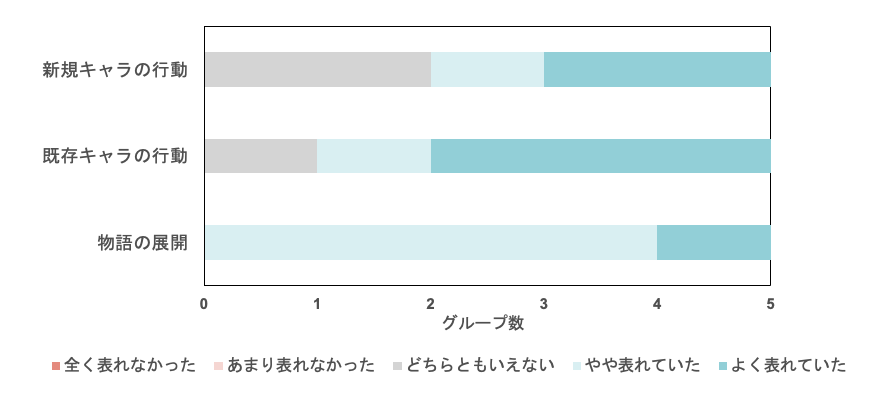
\includegraphics[width=12cm]{pict/05/similarity2.png}
   \caption[制作されたプロットにおける『ブラック・ジャック』らしさ]{制作されたプロットにおける『ブラック・ジャック』らしさ \footnotesize 第3回目のアンケートにおける「『ブラック・ジャック』らしさをどの程度感じたか教えてください。」という質問に対する回答結果    \label{similarity2}}
   \end{center}
\end{figure}

次に, 制作されたプロットで『ブラック・ジャック』らしさが感じられた要素を自由に記述してもらったアンケート結果の一部を表\ref{tab:similarity2}に示す. 表\ref{tab:similarity2}より, 様々な要素で『ブラック・ジャック』らしさがプロットの中に表れていたことが分かる. また, 表\ref{tab:similarity}と比較すると, 台詞や具体的描写について言及している記述が増加していることが分かる. これより, プロット編集セクションの利用は, プロットに対し具体的な要素を組み込むことを可能とし, さらにそれらを『ブラック・ジャック』らしい要素として表現することに寄与することが示唆される.

\vspace{1cm}

\setlongtables
\begin{tabularx}{12cm}{X}
   \caption[制作されたプロットで『ブラック・ジャック』らしさが感じられた要素の抜粋]{制作されたプロットで『ブラック・ジャック』らしさが感じられた要素の抜粋 \footnotesize 第3回目のアンケートにおける「『ブラック・ジャック』らしさがよく表れていた要素（物語展開やキャラの行動）があれば教えてください。」という質問に対する回答結果 \label{tab:similarity2}}
   \vspace*{3pt}
   \endfirsthead
   \hline
   \vspace{0.2cm}
   \begin{minipage}{\linewidth}
      \vspace{0.1cm}
         \begin{itemize}[itemsep=0pt, parsep=2pt]
            \item 新規キャラについて:
               \begin{itemize}[itemsep=0pt, parsep=2pt]
                  \item 父と息子が、自然と相反する価値観を持つ人間として描かれていた。
                  \item 登場人物が葛藤をよく持ちがちで、葛藤のちに前向きな思考を持つところ。
                  \item 台詞
               \end{itemize}
         \end{itemize}
         \vspace{0.2cm}
   \end{minipage} \\
   \begin{minipage}{\linewidth}
      \vspace{0.1cm}
         \begin{itemize}[itemsep=0pt, parsep=2pt]
            \item 既存キャラについて:
               \begin{itemize}[itemsep=0pt, parsep=2pt]
                  \item ブラックジャックのセリフ
                  \item ブラックジャックが、クールでありながら人の熱意に弱いところ。
               \end{itemize}
         \end{itemize}
         \vspace{0.5cm}
   \end{minipage} \\
   \begin{minipage}{\linewidth}
      \vspace{0.1cm}
         \begin{itemize}[itemsep=0pt, parsep=2pt]
            \item 物語の展開について:
               \begin{itemize}[itemsep=0pt, parsep=2pt]
                  \item どう書き換えても、手術は必ず成功した。
                  \item 患者の懇願、また手術後の喜びの描写が他の箇所よりもリアルに思えた。
               \end{itemize}
         \end{itemize}
         \vspace{0.1cm}
      
   \end{minipage}\\
   \hline
\end{tabularx}

次に『ブラック・ジャック』らしくないと感じられた要素について尋ねたアンケート結果の一部を示す. 「ブラック・ジャックらしくない要素が出されたが、それは採用せず、別の提案をAIに求めた。」や「初めに出してきたのは、「ブラックジャックらしくない」というよりも「物語としてまだなりたってない」要素が多かったので、そこの方が気になりました。」などの回答がその結果である. これより, 本システムから生成されるプロットは『ブラック・ジャック』らしくない要素やプロットとして満足のいかない要素を持つ場合があると分かる. 一方で, そのような要素が出力されていたとしても, 図\ref{similarity2}から分かるとおり『ブラック・ジャック』らしさは概ね良いとされており, また, 「別の提案を求めた」という記述があることからも, プロット編集セクションの利用によるインタラクティブな操作がそれらを排除することに寄与していたことが分かる. これは, 本システムにおいて実装したインタラクティブなLLMの操作が, 物語創作において有用であることを示唆する結果であるといえる.

\subsubsection{制作されたプロットの満足度}
制作されたプロットにおける, 各項目に関するクオリティについて尋ねたアンケート結果を図\ref{quality2}に示す. 図\ref{quality2}より, いずれのグループからも総合的な面白さや内容の幅広さについて高い満足度が見られ, 図\ref{quality}に示した結果と比較してもこれらの項目で良い回答が増加していることが分かる. これは, プロット編集セクションにおいて実装したLLMをインタラクティブに活用するプロット編集機能が, 内容の幅広さや面白さを高めることに寄与することを示唆する結果であるといえる. 一方で, 思いつかない展開であることや新規性といった面では悪いという回答も見られる. 新規性や思いつかない展開が生成されていないとみなされたことは, 出力が学習データに依存する LLM を創造的活動に用いる上で生じる課題の一つの表れであるといえる. また, 一貫性においても悪い評価が見られ, 図\ref{quality}に示した結果と比較してもその支持は低下していることが分かる. これは, プロット編集セクションの利用において, 部分的な修正を施すうちに, 物語の一貫性が損なわれてしまう場合があることを示唆する結果であるといえる. LLM とのインタラクティブな共創を促す上で重要な課題の一つであると考える.

\begin{figure}[H]
   \begin{center}
   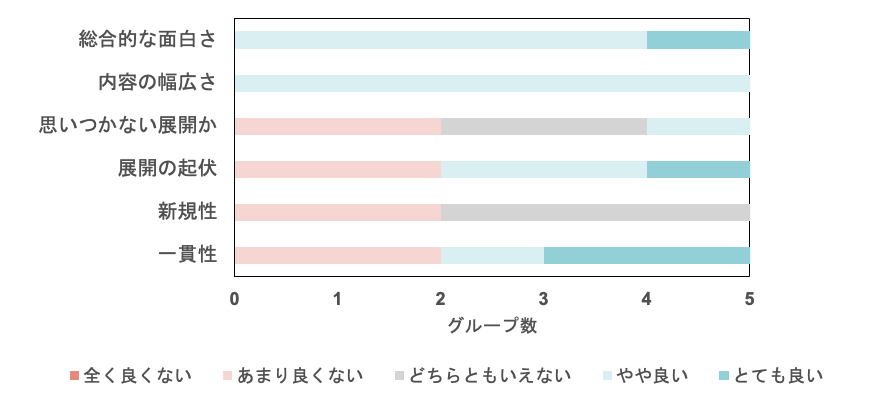
\includegraphics[width=12cm]{pict/05/quality2.png}
   \caption[制作されたプロットに対するクオリティの満足度]{制作されたプロットに対するクオリティの満足度 \footnotesize 第3回目のアンケートにおける「物語としてのクオリティについて評価してください。」という質問に対する回答結果 \label{quality2}}
   
   \end{center}
\end{figure}

次に, 本システムのインタラクティブ性について言及されたアンケート結果の一部を表\ref{tab:interaction}に示す. 表\ref{tab:interaction}より, 本システムにおけるインタラクティブ性が, 満足のいくプロットへの改善に効果的であったとみなされていることが分かる. これは, 本システムのインタラクティブなLLMの活用手法が, 物語創作において有用であることを示唆する結果であるといえる.

\setlongtables
\begin{tabularx}{12cm}{X}
   \caption{インタラクティブ性について記述されたアンケート結果の抜粋}
   \label{tab:interaction}
   \vspace{-3pt}
   \endfirsthead
   \hline
   \vspace{0.2cm}
   \begin{minipage}{\linewidth}
      \vspace{0.1cm}
               \begin{itemize}[itemsep=0pt, parsep=2pt]
                  \item AIが1人で作ったというよりも、一緒に何回も変えていった感覚が強いので、AI単体の評価となると難しくなる。
                  \item 初めにAIが出してきたものの評価となるともっと低くなるし、最終形態とするともっと高くなります。
                  \item 最初は、展開が一定でした。でも、修正を重ねる中でどんどん良くなってくれるので、結果とても良いと思います。
                  \item 一貫性など、全てAIが兼ね備えていた訳ではなく、個々に修正（AIに質問して正い方向を導き出す）したことで得られた。
               \end{itemize}
   \end{minipage} \\
   \hline
\end{tabularx}

\subsubsection{制作されたプロットの制御性}
プロット編集セクションの利用も含め, 本システムを通じ入力した内容や選択した内容がプロットにどれだけ反映されたか, その反映具合について尋ねたアンケート結果を図\ref{control2}に示す. 図\ref{control}に示した結果と比較すると, テーマ, ジャンルの項目について高い評価が増加していることが分かる. これは, 本システムのプロット編集セクションにおける機能が, ユーザーが思い描くテーマやジャンルを具体化することに寄与することを表す結果であるといえる. 図\ref{control2}より, 物語構造, 登場人物に関する項目も高い評価を得ており, このことから物語構造分析の活用は, プロット編集セクションにおいて提供した LLM とのインタラクティブな共創手法にも通じて物語の生成に有益であると考えられる.

%本システムのプロット編集セクションによる改善作業により, 単に一度生成されただけのプロットが, 自身の思い描くテーマやジャンルに沿う物語として具体的にプロットとして実現されるよう寄与したことを表す結果であるといえる.


\begin{figure}[H]
   \begin{center}
   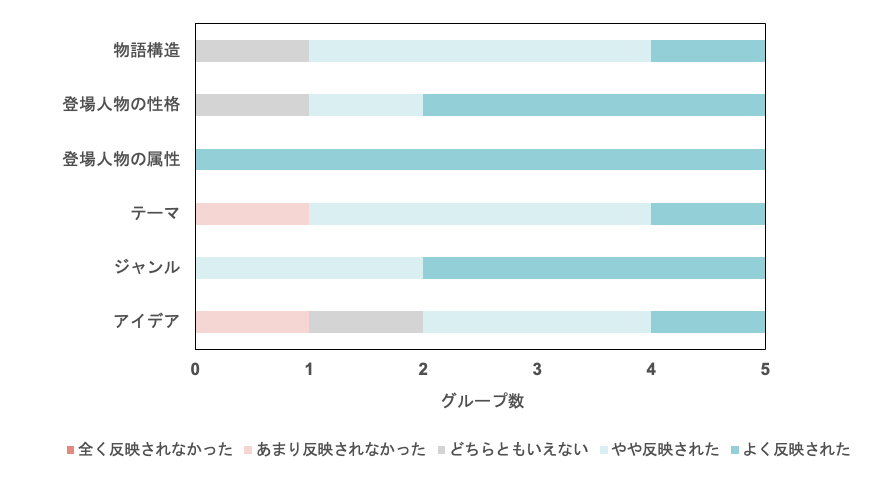
\includegraphics[width=12cm]{pict/05/control2.png}
   \caption[プロットの制御性に関するアンケート結果]{プロットの制御性に関するアンケート結果 \footnotesize 第3回目のアンケートにおける「入力内容が出力プロットにどれほど反映されたと感じますか？」という質問に対する回答結果 \label{control2}}
   \end{center}
\end{figure}

\subsubsection{プロット編集セクションの効果}
プロット編集セクションにおける各項目について尋ねたアンケート結果を図\ref{edit}に示す. 図\ref{edit}より, プロット編集セクションの利用は, 面白さへの貢献と, 指示の反映, いずれの項目についても高く評価されていることが分かる. これは本システムのプロット編集セクションにおける LLM とのインタラクティブな共創手法が物語の創作において有益であったことを示唆する結果であるといえる.

\begin{figure}[H]
   \begin{center}
   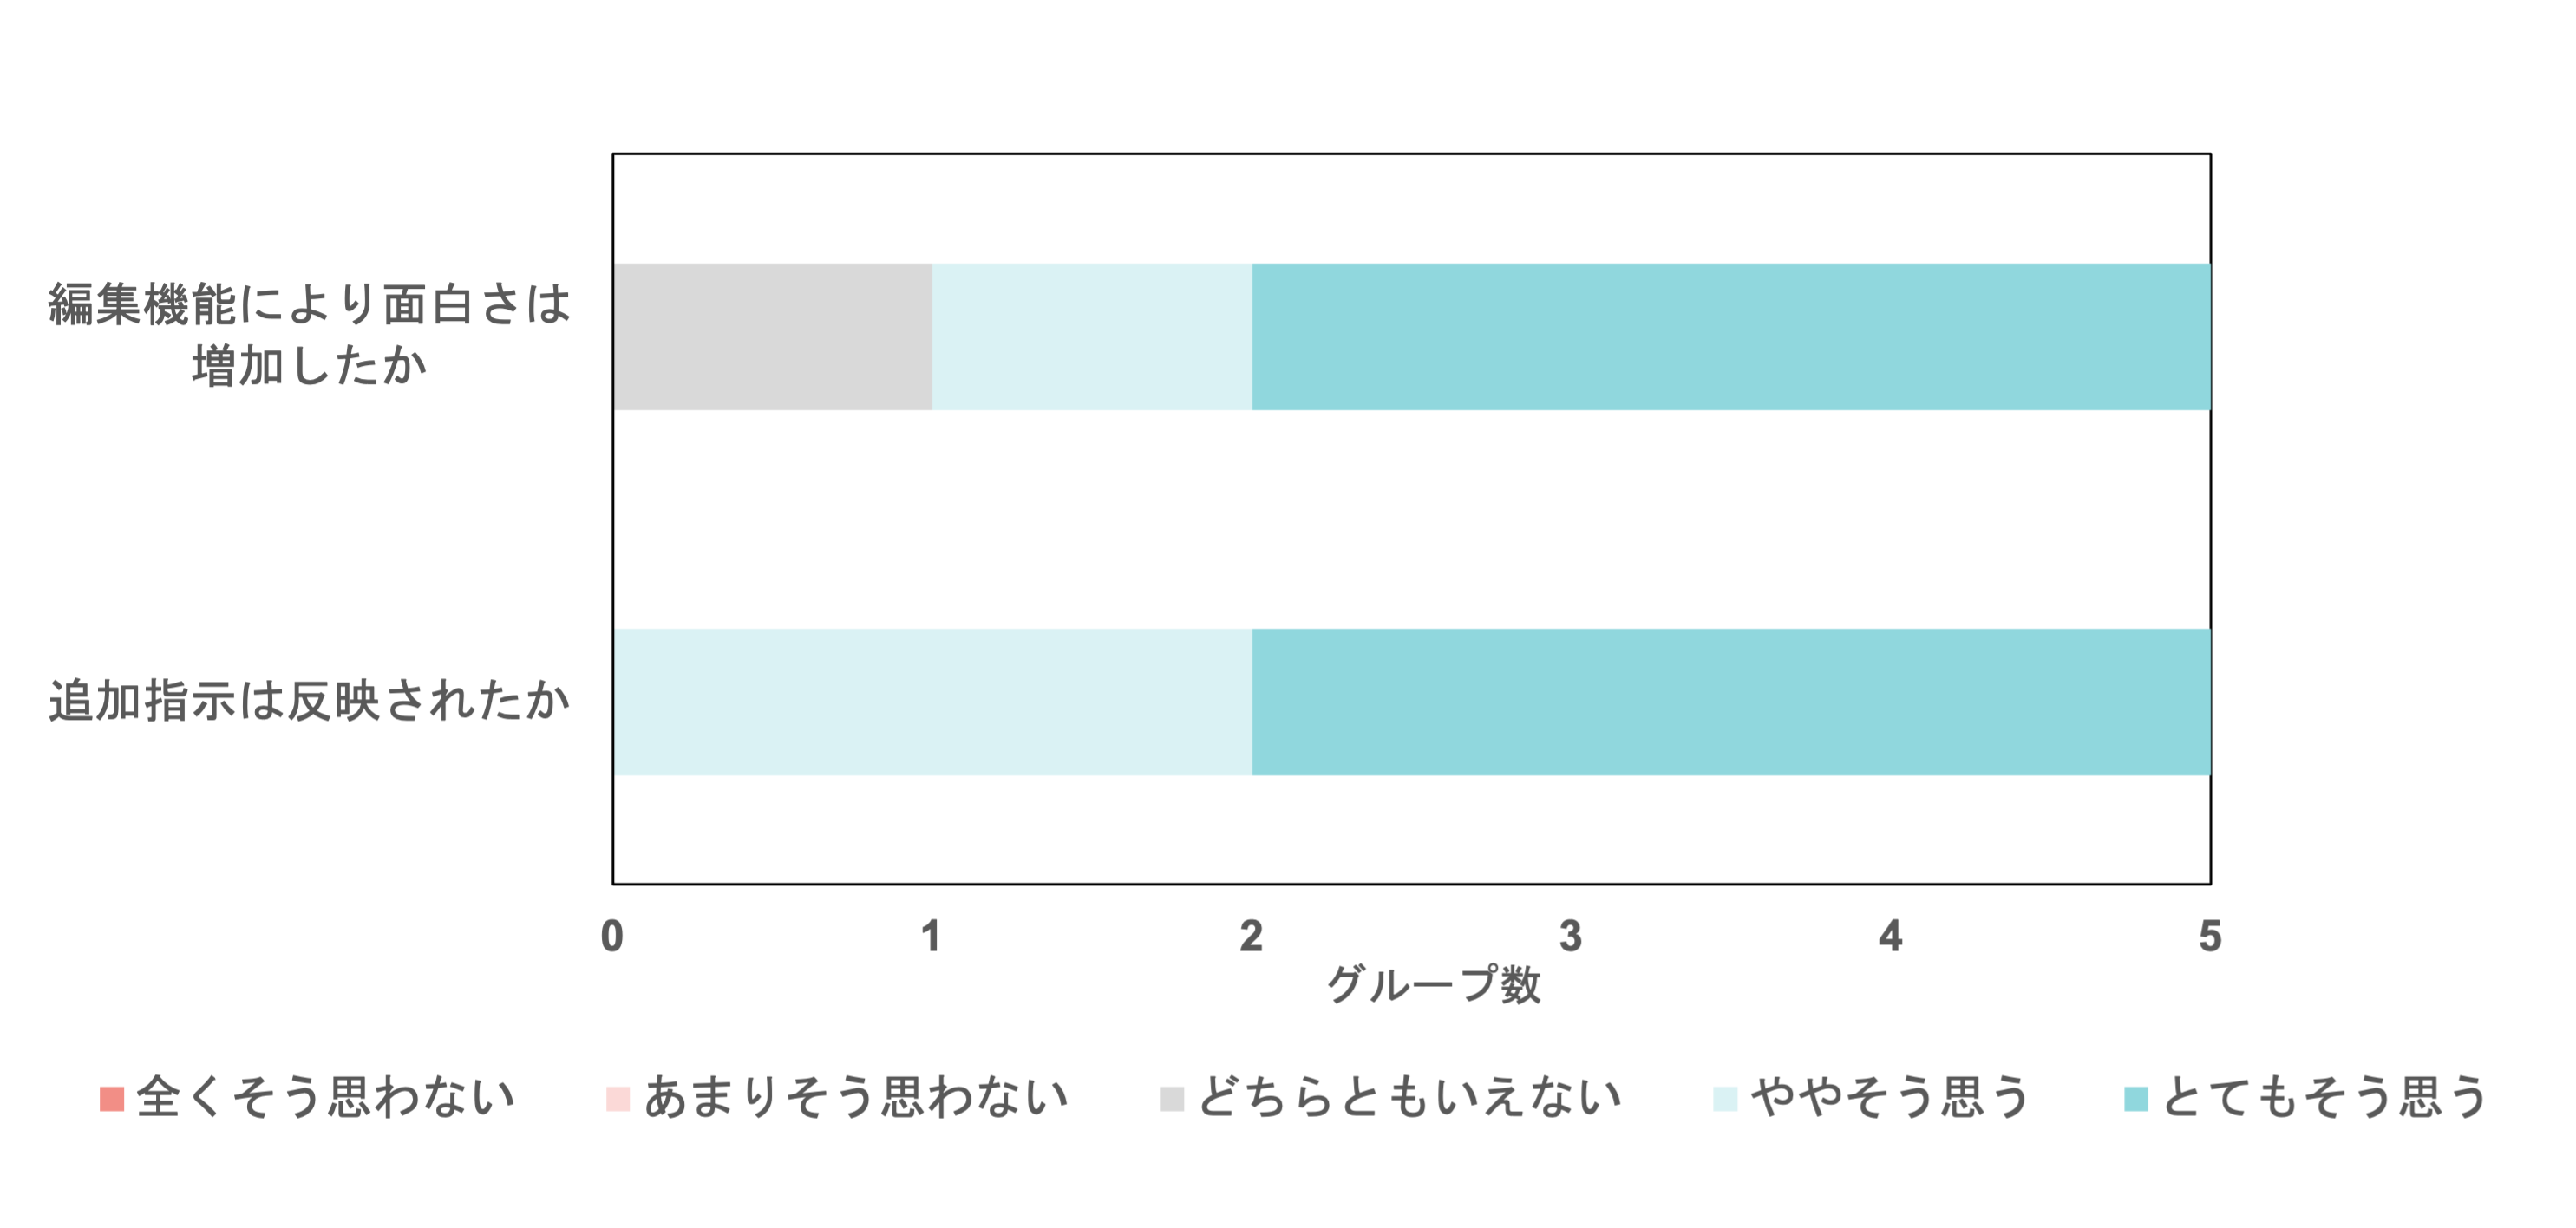
\includegraphics[width=12cm]{pict/05/edit.png}
   \caption[プロット編集セクションにおける満足度]{プロット編集セクションにおける満足度 \footnotesize 第3回目のアンケートにおける「編集作業の結果、こちらのプロットは面白くなったと感じますか？」という質問と「追加指示が適切に反映されたか？」に対する回答結果 \label{edit}}
   \end{center}
\end{figure}

\subsubsection{創作活動における利便性}
本システム全体の利用を通じ, 創作支援としての貢献度ついて尋ねたアンケート結果を図\ref{comfortable}に示す. 図\ref{comfortable}より, 本システムが操作性については十分に良いものとして受け入れられた一方で, 作業時間の短縮という側面では満足が得られなかったという回答もあり, 十分な貢献ができていなかったことが分かる. また, 創造性の刺激については低い評価を受けることはなかったものの, まずまずの評価に留まっていることが分かる.

操作性について高い満足度を得たことは, 本システムにおいて実装された選択と入力を基本とする操作がストーリークリエーターにとり, 直感的で使いやすいものであったことを示唆する結果であるといえる. 一方で, 作業時間の短縮については, LLM からのレスポンスの遅さに不満の声が聞かれ, より高速に応答する LLM がこの問題を解決すると考えられる. 創造性への刺激については, まずまずの評価を得ているが, 生成されるプロットのクオリティにおいて, 十分に満足を与えることができなかった目新しさや幅広さの提供に取り組むことで, さらなる貢献をもたらすことができるようになると考えられる.

\begin{figure}[H]
   \begin{center}
   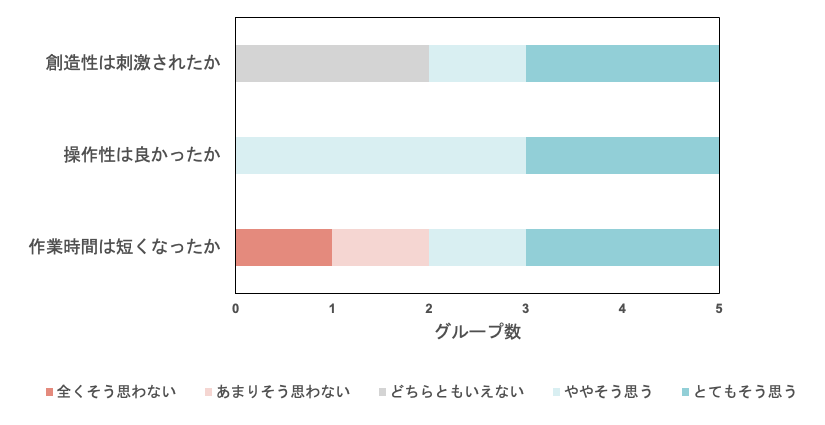
\includegraphics[width=12cm]{pict/05/comfortable.png}
   \caption{本システムの創作支援における満足度}
   \label{comfortable}
   \end{center}
\end{figure}

\section{ログの結果および考察}\label{log}

ここでは, プロジェクトの全肯定にわたり得られた本システムの操作ログデータの分析結果を示し, 本システムの創作支援における貢献について考察する.

なお, ログの分析においては, 筆者と他１名の学生で取り組んだ.

\subsection{作業時間}
プロット制作という創造的活動の作業時間を正確に把握することは難しい. 実際に手を動かしていなくとも, アイデアや構想を練ることなどに時間は使われるからである. 一方で創作活動の時間効率性を高めることは, 創作支援の重要な項目の一つであると考えられる. よって本論文では, 本システムの操作ログより作業時間を概算し, 本システムの時間効率への寄与について考察する.


操作ログデータとして得られた本システムのボタン押下間隔の度数分布を図\ref{time_f}に示す. 図\ref{time_f}より, ボタン押下間隔とその度数には冪乗則が成立しているように見られる. そこで, 創作活動中のボタン押下間隔は冪乗則に従うと仮定し, どこまでのボタン押下間隔が, 創作活動中のものか求めることとした. つまり, 創作活動中最後のボタン押下と, 創作活動から離れ再び戻ってきた時のボタン押下の間隔は, 冪乗則を崩す原因となると仮定した. そこで, このグラフを両対数グラフへと変換した上で直線近似を行い, その決定係数を求めた. その結果を図\ref{time_r}に示す. これは, 0 hから始まりどこまでのボタン押下間隔が最も決定係数を大きくするか求めたもので, 横軸はその閾値を表す. 図\ref{time_r}より, ボタン押下間隔のデータを0.00 hから0.89 hまでの範囲で直線近似すると, 決定係数が最大値 0.57 をとることが分かった.

\begin{figure}[H]
   \begin{center}
   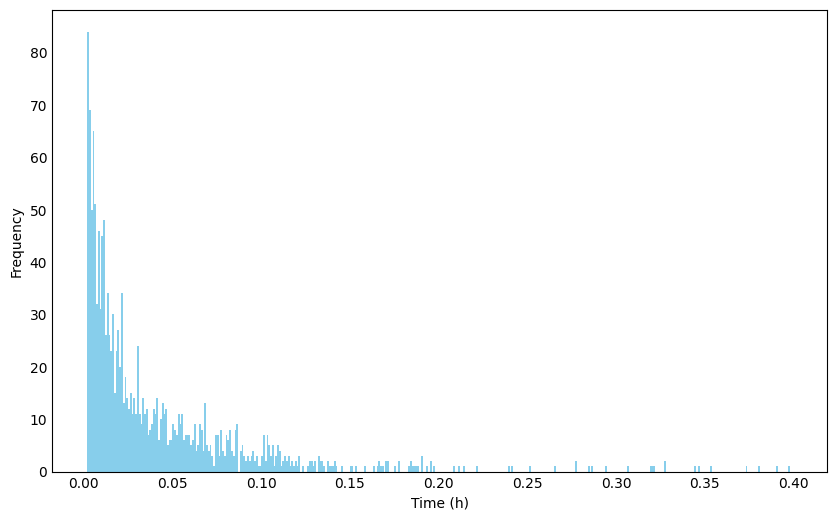
\includegraphics[width=10.5cm]{pict/05/time_f.png}
   \caption[ボタン押下間隔の度数分布]{ボタン押下間隔の度数分布. 階級幅は0.001 h}
   \label{time_f}
   \end{center}
\end{figure}

\begin{figure}[H]
   \begin{center}
   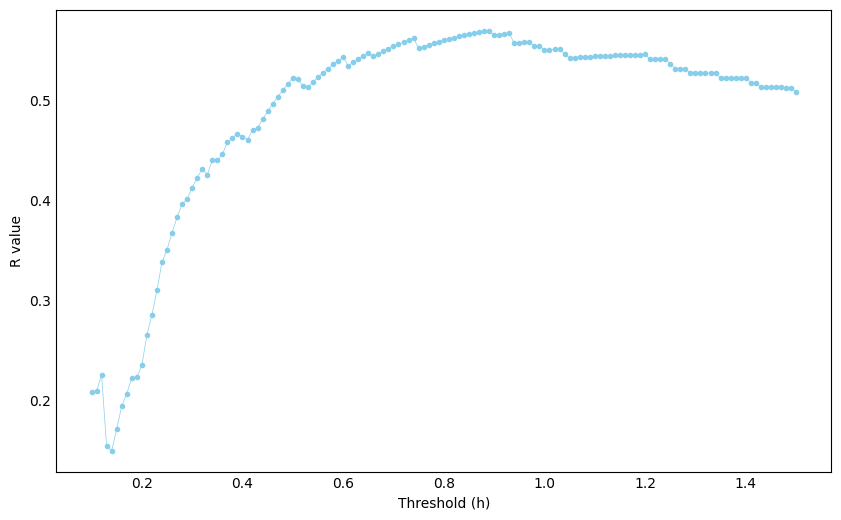
\includegraphics[width=10.5cm]{pict/05/time_r}
   \caption[ボタン押下間隔における閾値と決定係数の関係]{ボタン押下間隔における閾値と決定係数の関係. \footnotesize 閾値が 0.89 h であるとき決定係数は最大値 0.57 をとる.}
   \label{time_r}
   \end{center}
\end{figure}

一般に, 休憩時間と称し作業から離れる場合, キリの良い時間が採用される. 図\ref{time_r}より, データを集める閾値を 1.00 h とした場合, 決定係数は 0.55 であり最大値に接近した値である. そこで, 本論文では, ボタン押下間隔が 1.00 h 以上開いている値は作業時間に含めずに, ボタン押下間隔が 1.00 h 未満の値を全て足し上げ算出した値を便宜的に作業時間とみなすこととした. なお, 1.00 h は集計されたボタン押下間隔のうち, 98 パーセンタイルから 99 パーセンタイルの間に位置する値であり, このことも 1.00 h を閾値とすることに整合性を保たせる理由であると考える.

概算した作業時間を図\ref{time}に示す. グループAにおいては, プロット制作期間内に2つのプロットを制作したため作品ごとに作業時間を集計した. 図\ref{time}より, グループC は最も長く制作時間を費やしたグループであり, グループEは最も短い時間でプロット制作を行ったグループであることが分かる.

図\ref{comfortable}に示した「作業時間が短くなったか」 というアンケートへの回答のうち「短くなったとは思わない」と回答したのは, グループ C と E であり, そのほかのグループは「短くなったと思う」と回答している.

\begin{figure}[H]
   \begin{center}
   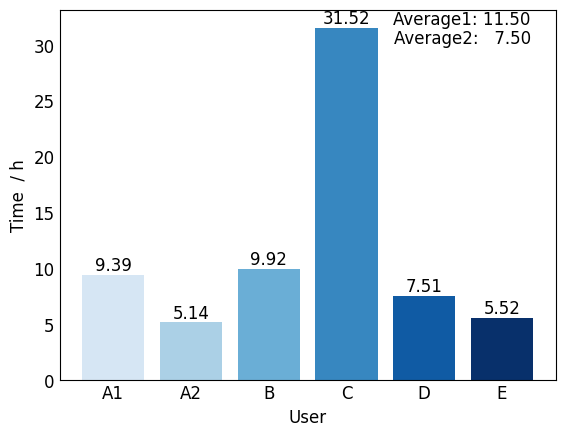
\includegraphics[width=10cm]{pict/05/time}
   \caption[作業時間の概算結果]{タンの押下間隔から算出した作業時間. グループAは制作期間内において2つのプロットを制作したため作品ごとに作業時間を集計した. Average1 は全体平均, Average2 は外れ値を除いた平均値を表す.}
   \label{time}
   \end{center}
\end{figure}

作業時間の最も短いグループ E が作業時間の短縮を感じなかったのは, LLM の応答の遅さや, 自身のプロット制作にかかる時間が元々十分に早いことなどが理由にあると考えられる. 一方で, 最も時間をかけたグループCが作業時間の短縮を感じなかったのは順当な結果であるといえる. 

ここで, それぞれのグループが編集機能をどれだけ利用したかその回数を表\ref{tab:edit}に示す. 表\ref{tab:edit}より, グループCは最も編集機能を利用したグループであることが分かる. これは, グループCがプロット制作に最も多くの時間を費やしていることと整合的であるといえる. また, 作業時間の短縮を感じさせることができなかった要因の一つとして編集機能における操作性や応答の質, 速さについて解題があるとも考えられる.

\begin{table}[H]
\begin{center}
{\caption{各グループの編集機能の利用数}
\label{tab:edit}
\begin{tabular}{ccccc} \hline
A & B & C & D & E  \\ \hline
116 & 60 & 176 & 33 & 45\\
\hline
\end{tabular}
}
\end{center}
\end{table}

一方で, 作業時間の短縮を感じられたと回答したグループはいずれも作業時間が 10 時間未満であり, このことに本システムの時間効率への寄与があったのではないかと考えられる. 一般にプロット制作における作業時間が何時間であるかは人に依るところが大きいとされているが, 参加者からは「自分一人でやるよりも断然早いと」いった声も聞かれ, プロット制作を 10 時間未満で終えられたことは比較的早く作業を終えられたことを意味し, 本システムがもたらした効率性の高さを示唆する結果であるとも考えられる.

\subsection{プロット編集セクションの利用}\label{subsec: edit_result}
プロット編集セクションにおける機能が, それぞれどれだけ利用されたかその回数をまとめたものを表\ref{tab:edit_count}に示す. またその全体の利用率を図\ref{edit_c}に, グループごとに正規化した利用率を図\ref{edit_c2}に示す. 表\ref{tab:edit_count}および図\ref{edit_c}, 図\ref{edit_c2}より, プロット編集セクションに実装した機能の中で, 自由記述による指示や質問を行うことができる\hyperref[subsec: freeword]{フリーワードによるやり取り}機能が最も多く利用されていたことが分かる. 特に, グループCの作業時間や編集機能の利用回数の大きさを考慮し, このグループの利用率が支配的にならぬようグループごとに正規化した利用率においても, フリーワードによるやり取り機能の利用率 50 \% を超えている. この結果から, 生成されたプロットが型にはまらない自由な発想を引き出した可能性や, プロのストーリークリエーターが自身の言葉による制御を望んていたこと, プロットの多様性により, 機能を限定しない編集が必要となっていたことなどが考えられる. また, 次に利用回数の多い機能が\hyperref[subsec: question]{プロット中の単語・文章に関する質問}機能であり, \hyperref[subsec: freeword]{フリーワードによるやり取り}機能においてもプロットへの質問を行うことができることを踏まえ, プロット編集セクションにおける質問機能が重要であったことが分かる. これは, LLM とのインタラクティブな共創手法として, 創作物に対する質問とその応答, その応答の利用を促すシステムが有用であることを示唆する結果であるといえる.

\begin{table}[H]
   \begin{center}
   \caption{各編集機能の利用回数}
   \label{tab:edit_count}
   \begin{tabular}{lr} \hline
   編集機能 & 利用された回数 \\ \hline
   一部シーン変更 & 12 \\
   フリーワードによるやり取り & 271 \\
   アイデア生成 & 21 \\
   手作業での編集 & 47 \\
   プロット中の単語・文章に関する質問 & 32 \\
   その他 & 47 \\
   \hline
   \end{tabular}
   \end{center}
   \end{table}

\begin{figure}[H]
   \begin{center}
   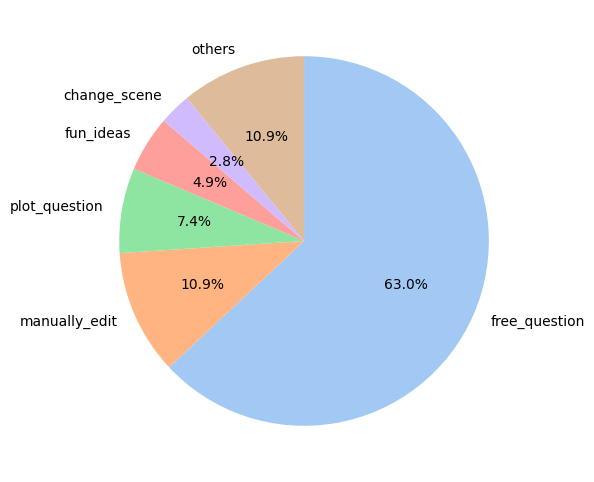
\includegraphics[width=10cm]{pict/05/edit_c}
   \caption[プロット編集セクションにおける編集機能の利用率]{プロット編集セクションにおける編集機能の利用率}
   \label{edit_c}
   \end{center}
\end{figure}

\begin{figure}[H]
   \begin{center}
   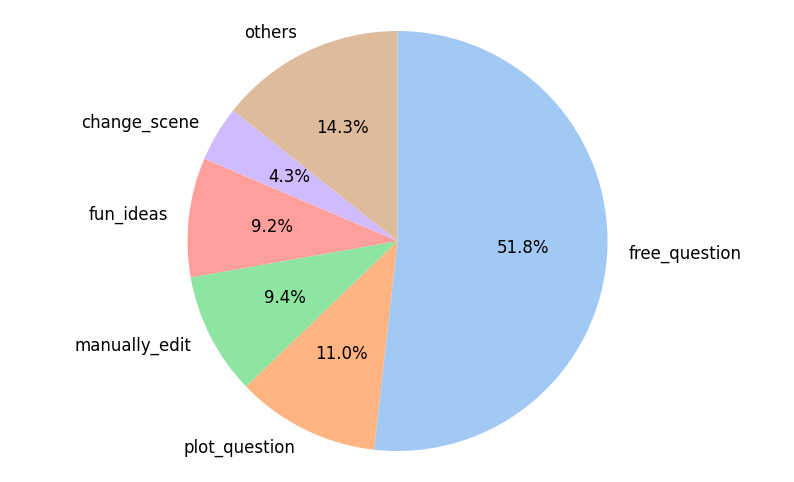
\includegraphics[width=10.5cm]{pict/05/edit_c2}
   \caption[プロット編集セクションにおける編集機能の利用率(正規化)]{プロット編集セクションにおける編集機能の利用率(正規化)}
   \label{edit_c2}
   \end{center}
\end{figure}
 
\subsection{プロット編集セクションにおいて生成されたプロットの採用率}

プロット編集セクションにおける編集機能を用いることで新たに生成されたプロットが既存のプロットに比べどれだけ採用されたかその採用率を表\ref{tab:adopt}に示す. 表\ref{tab:adopt}より, 編集機能により生成された新たなプロットはいずれのグループにおいても 65 \% 以上の採用率であり, 全体を通して高い採用率であることが分かる. この結果は, 図\ref{edit}示したアンケート結果, 「編集機能により面白さは増加したか」という問において高い評価が得られた結果と符合している. つまり, これらの結果は, LLM とのインタラクティブなプロット創作を可能とする本システムの編集機能が, プロットの質向上に寄与することを示唆する結果であるといえる.

% \begin{figure}[H]
%    \begin{center}
%    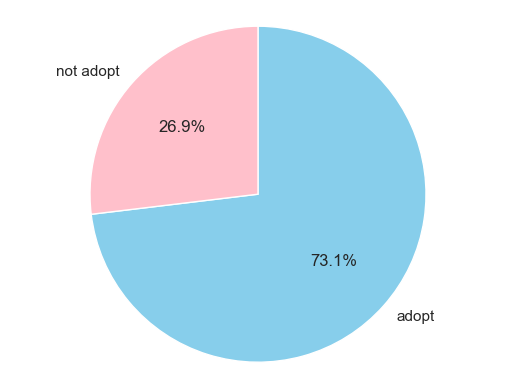
\includegraphics[width=12cm]{pict/05/adopt_c1.png}
%    \caption{プロット編集セクションにおいて生成されたプロットの採用率}
%    \label{adopt_c1}
%    \end{center}
% \end{figure}

% \begin{figure}[H]
%    \begin{center}
%    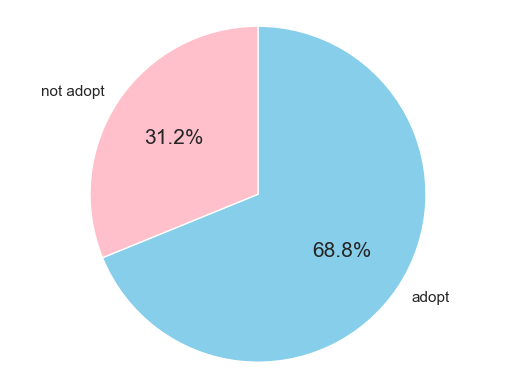
\includegraphics[width=12cm]{pict/05/adopt_c2.png}
%    \caption{プロット編集セクションにおいて生成されたたプロットの採用率(正規化)}
%    \label{adopt_c2}
%    \end{center}
% \end{figure}

% プロット編集セクションにおいて生成されたプロットは, いずれのグループにおいても 50 \% 以上採用されたことが分かる. これは, プロット編集セクションにおける編集機能が, 生成されたプロットをより満足のいくものへと改善することに寄与することを示唆する結果であるといえる.

\begin{table}[H]
   \begin{center}
   \caption{プロット編集セクションにおいて生成されたプロットの採用, 不採用}
   \label{tab:adopt}
   \begin{tabular}{cccccccc} \hline
   & A & B & C & D & E & Total & mean \\ \hline
   採用率 & 0.75 & 0.91 & 0.71 & 0.69 & 0.67 & 0.75 & \textbf{0.74}\\
   採用数 & 21 & 50 & 101 & 11 & 18 & 201 & -\\
   非採用数 & 7 & 5 & 41 & 5 & 9 & 67 & -\\
   \hline
   \end{tabular}
   \end{center}
   \begin{tablenotes}
   \footnotesize
   \item 「Total」は全選択数における採用数の割合を表す.
   \item 「mean」はグループごとの採用率の平均を表す.
   \end{tablenotes}
\end{table}

\section{提案手法の成果}\label{self_result}
ここでは執筆者の提案手法である, タイトルとあらすじの生成機能の成果について述べる.

「TEZUKA2023」プロジェクトにおいて制作された『ブラック・ジャック』の新作エピソードは, そのタイトルを『機械の心臓-Heartbeat Mark \MakeUppercase{\romannumeral 2} \footnotemark』として週刊少年チャンピオンに掲載されることとなったが, このタイトルにある「機械の心臓」という言葉は提案手法, タイトルの生成において出力された言葉である. つまり, タイトルの生成は商業的なレベルの出力が可能であることが分かった. また, タイトルの生成で出力された「機械の心臓」をプロットの設定として入れ込み, プロット生成を行った結果, プロット本文内で Heartbeat Mark \MakeUppercase{\romannumeral 2}という言葉が出力された. クリエーターはこの言葉を中心として物語を想起し, 新作エピソードとしてのシナリオを完成させていた. タイトルという作品全体に影響を与える要素の生成は, クリエーターの創作支援において重要な役割を果たす可能性が示唆されたと考えられる.
\footnotetext{\url{https://keio.app.box.com/s/i1kdiunyr3o94ud6r2h701v4xumahgjx} (cited 2024-01-28)}

% プロット編集セクションにおける編集機能が, 編集機能ごとにどれだけ利用されたか, その回数を被験者グループごとにまとめものを図\ref{edit_g}に示す. 図\ref{edit_g}より, 

% \begin{figure}[H]
%    \begin{center}
%    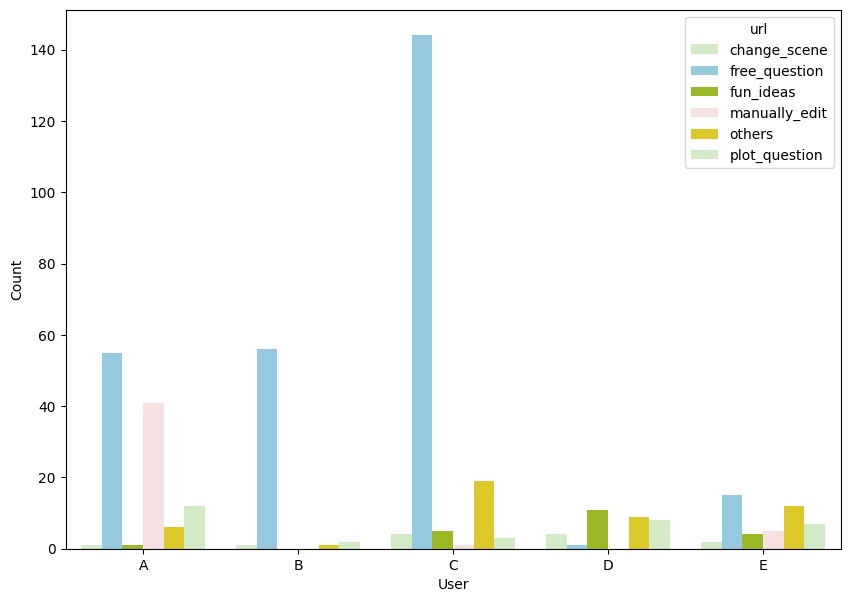
\includegraphics[width=12cm]{pict/05/edit_g}
%    \caption[プロット編集セクションにおける編集機能の利用回数]{プロット編集セクションにおける編集機能の利用回数}
%    \label{edit_g}
%    \end{center}
%\end{figure}

% \subsection{生成されたプロットに対する満足度}

% 図\ref{quality}より, 本アプリケーションは, 目新しさの提供に課題がある一方で, 幅広さや面白さといった観点で, プロのストーリークリエーターから見ても創作活動に役立つものであったことがわかる.

% 複合的な作品である『ブラック・ジャック』の分析データを, プロットの生成に活用したことが, LLM に幅広い言葉の出力を促したのではないかと考えられる.

% 一方, 目新しさの課題については, 出力が学習データに制限される LLM を創造的活動に用いる上で重要な課題の一つであるといえる.

% \subsection{LLM との共創における貢献度}

% 図\ref{qc}より, 作業時間の短縮に関する貢献を除き, 低い評価を受けていないことがわかる. 特に, 使いやすさと指示の反映に関する項目について高い評価を受けており, 本アプリケーションが LLM との創作活動を向上させる可能性を示唆した結果であるといえる.

% 作業時間については, LLM からのレスポンスの遅さに不満の声が聞かれ, より高速に応答する LLM がこの問題を解決すると考えられる.

% 創造性への刺激については, まずまずの評価を得ているが, 目新しさを提供する課題の取り組みにより, さらなる貢献をもたらすことができると考える.

% \section{ログの結果および考察}

% \subsection{作業時間}
% プロット制作という創造的活動の作業時間を正確に把握することは難しい. 実際に手を動かしていなくとも, アイデアや構想を練ることなどに時間は使われるからである. 一方で創作活動の時間効率性を高めることは, 創作支援の重要な項目の一つであると考えられる. よって本論文では, 本アプリケーションの操作ログより作業時間を概算し, 本アプリケーションの時間効率への寄与について考察する.


% 作業時間は, ログデータとして集計した, 本アプリケーション画面のボタン押下間隔のうち, 98 パーセンタイルから 99 パーセンタイルの間に位置する 1 時間を区切りとして算出した. つまり, ボタン押下間隔が 1 時間以上開いている値は作業時間に含めずに, ボタン押下間隔が 1 時間未満の値を全て足し上げ算出した値を便宜的に作業時間とみなすこととした.

% 図\ref{qc}で示した, 「作業時間が短くなったか」 というアンケートへの回答のうち「短くなったとは思わない」と回答したのは, グループ C と E であり, そのほかのグループは「短くなったと思う」と回答している. 図\ref{time}からわかる通り, グループ C は作業時間を最も費やしたグループである一方, グループ E は最も作業時間の少ないグループであった.

% グループ E が作業時間の短縮を感じなかったのは, LLM の応答の遅さや, 自身のプロット制作にかかる時間が元々十分に早いことなどが理由であると考えられる. 

% \begin{table}[hbtp]
% \small
% \begin{center}
% {\caption{各グループの編集機能の利用数}
% \label{edit_action}
% \begin{tabular}{ccccc} \hline
% A & B & C & D & E  \\ \hline
% 116 & 60 & 176 & 33 & 45\\
% \hline
% \end{tabular}
% }
% \end{center}
% \end{table}

% 表\ref{edit_action}に示した通り, グループ C は最も多く編集機能を用いたグループでもある. これより, 編集機能における操作性などが時間効率に影響していると考えられる.

% 一方で, 作業時間の短縮を感じられたと回答したグループはいずれも作業時間が 10 時間未満であり, このことに本アプリケーションの時間効率への寄与があったと考えられる.

% \subsection{編集機能により生成したプロットの採用率}


% \begin{table}[hbtp]
% \begin{center}
% {\caption{グループごとの編集機能により生成したプロットの採用率とそれらの平均}
% \label{adopt_t}
% \begin{tabular}{cccccc} \hline
% A & B & C & D & E  \\ \hline
% 0.71 & 0.91 & 0.70 & 0.50 & 0.63\\
% \hline
% \end{tabular}
% }
% \end{center}
% \end{table}
% 表\ref{adopt_t}より, 編集機能を用いて, 既存のプロットを新たなプロットへと書き換えた際, ほとんどのグループで新旧プロットのうち新しいプロットを採用する割合が大きいことがわかる. 各グループの採用率の平均もおよそ 70 \% と高い割合を示している. 

% この結果は, 表\ref{qc}で示したアンケート結果, 「編集機能により面白さは増加したか」という問において高い評価が得られた結果と符合している. つまり, これらの結果は, LLM とのインタラクティブなプロット創作を可能とする本アプリケーションの編集機能が, プロットの質向上に寄与することを示唆する結果であるといえる.

% % \begin{figure}[htbp]
% % \begin{center}
% % 
\includegraphics[width=70mm]{img/5/comparison.png}
% % \caption{編集機能により生成したプロットの採用・不採用数}
% % \label{adopt}
% % \end{center}
% % \end{figure}

% \subsection{用いられた編集機能の割合}


% 図\ref{edit_action}より, 編集機能の中でフリーワードでやり取りする機能が最も多く利用され, グループごとに正規化した利用率の中でも50\%以上を占めることがわかる. 

% この結果から, 生成されたプロットが, 型にはまらない自由な発想を引き出した可能性や, プロのストーリークリエーターが自身の言葉による制御を望んていたこと, プロットの多様性により, 機能を限定しない編集が必要となっていたことなどが考えられる.

% フリーワードでのやり取りに対する支援の拡充が求められていると考える.

\expandafter\ifx\csname ifdraft\endcsname\relax
\fancyhead[LO]{}
\printbibliography[title=参考文献]
\end{document}
\fancyhead[LO]{\rightmark}
\fi